%%%%%%%%%%%%%%%%%%%%%%%%%%%%%%%%%%%%%%%%%
% Original author:
% Linux and Unix Users Group at Virginia Tech Wiki
% (https://vtluug.org/wiki/Example_LaTeX_chem_lab_report)
% Modified by: Hector F. Jimenez S, for the Digital Electronics Laboratory.
% License:
% CC BY-NC-SA 3.0 
%%%%%%%%%%%%%%%%%%%%%%%%%%%%%%%%%%%%%%%%%
%----------------------------------------
%	PACKAGES AND DOCUMENT CONFIGURATIONS
%---------------------------------------
\documentclass[paper=a4, fontsize=12pt]{article} 		% A4 paper and 11pt font size
\usepackage[T1]{fontenc} 								% Use 8-bit encoding that has 256 glyphs
%\usepackage{fourier}		 							% Use the Adobe Utopia font for the document 
\usepackage[spanish,english]{babel}						% Spanish Language, templates uses some sections in english.
\selectlanguage{spanish}								% main language.
\PassOptionsToPackage{spanish}{babel}
%\renewcommand{\figurename}{Figura}						% Force rename of figure.
%\renewcommand{\figurename}{Fig.}
\usepackage[figurename=Fig.]{caption}
\usepackage[utf8]{inputenc}								% tildes for spanish language.
\usepackage{amsmath,amsfonts,amsthm} 					% Math packages.
\usepackage{minted}										% For syntax highlighting.
	    \renewcommand\listingscaption{Código}			%rename the source code minted !
\usepackage{float}										% Image will be in the same place as you want.!!! x-/
\usepackage{sectsty} 									% Allows customizing section commands
\allsectionsfont{\centering \normalfont\scshape}	   	% Make all sections centered, the default font and small caps
\usepackage{hyperref}
\hypersetup{											%Setups the false color and borders.
    colorlinks=false,
    pdfborder={0 0 0},
}
\newcommand\fnurl[2]{%									% set a simple and quick footnote command and include url.
\href{#2}{#1}\footnote{\url{#2}}%	
}
\usepackage{graphicx}									% Import easyly images.
\graphicspath{ {./images/} }							% Where to look for the images.
\DeclareGraphicsExtensions{.pdf,.png,.jpg}				% Graphics Extension to be used
\usepackage[notes,backend=biber]{biblatex-chicago}		% Bibliography and references.
\bibliography{biblio}									% bibliography filename.
\usepackage{fancyhdr} 									% Custom headers and footers
\pagestyle{fancyplain} 									% Makes all pages in the document conform to the custom headers and footers
\fancyhead{} 											% No page header
\fancyfoot[L]{} 										% Empty left footer
\fancyfoot[C]{} 										% Empty center footer
\fancyfoot[R]{\thepage} 								% Page numbering for right footer
\renewcommand{\headrulewidth}{0pt} 						% Remove header underlines
\renewcommand{\footrulewidth}{0pt} 						% Remove footer underlines
\setlength{\headheight}{13.6pt} 					    % Customize the height of the header
\numberwithin{equation}{section}						% Number equations within sections (i.e. 1.1, 1.2, 2.1, 2.2 instead of 1, 2, 3, 4)
%\numberwithin{figure}{section} 						% Number figures within sections (i.e. 1.1, 1.2, 2.1, 2.2 instead of 1, 2)
\numberwithin{table}{section} 							% Number tables within sections (i.e. 1.1, 1.2, 2.1, 2.2 instead of 1, 2, 3, 4)
\setlength\parindent{0pt} 								% Removes all indentation from paragraphs
\newcommand{\horrule}[1]{\rule{\linewidth}{#1}} 		% Create horizontal rule command with 1 argument of height
%%%%%%%%%%%%%%%%%%%%
%Title Section
%%%%%%%%%%%%%%%%%%%%%
\usepackage{tikz}										%Draw arrays. in tex.
\usetikzlibrary{matrix,backgrounds}

\usepackage{listings}% http://ctan.org/pkg/listings

\renewcommand{\lstlistingname}{Codigo}	


\title{Estructuras de Datos\\ 
\horrule{0.5pt} \\[0.4cm] 								% Thin top horizontal rule	Title rule
\textit{Vectores vs Arrays, Analisis de Algunas de sus Operaciones}
\horrule{1pt} \\[0.5cm] 			
} 			% Title

\author{												% Authors begin.
Héctor F. \textsc{Jiménez S.}\\
\texttt{hfjimenez@utp.edu.co} \\
\texttt{PGP KEY ID: 0xB05AD7B8}
\and
Cristian Camilo \textsc{Perilla C.}\\
\texttt{camilo980818@gmail.com }\\
} 
% End of  Author name
\date{}    						                       % Date for the report, this will hide the \today.

\begin{document}
\maketitle                      			           % Insert the title, author and date
\begin{center}
\begin{tabular}{l r}								   % two column to
Fecha de Entrega: & Septiembre, 2016 \\				   % Ramiro's Details.
Profesor: & Gustavo Adolfo Gutierrez Sabogal
\end{tabular}
\end{center}
%%%%%%%%%%%	
% Let's start the document.
%%%%%%%%%%%	
\section{Objetivos}
\begin{itemize}
   \item Identificar las ventajas y desventajas de los arrays y vectores.
  \item Identificar la complejidad de las operaciones realizadas sobre los arrays y vectores,como \textbf{add(), get(), remove(), insert()}.
  \item Realizar la implementacion y analisis en lenguaje C++11. 
\end{itemize}
En nuestro mundo de algoritmos vivimos y tratamos de subsistir para poder dar soluciones a una gran cantidad de problemas del mundo real, somos nosotros los que con ideas poderosas y abstractas las podemos convertir en magia para tratar esa gran cantidad de información que esta allí, sin importar el tipo de patrón, dato o complejidad es necesario darle el respeto adecuado a los datos, por ello las estructuras de datos existen para brindarles el mejor cariño y manipulación que nos permitan realizar un tratamiento correcto, eficiente y preciso en la medida posible. 

En este informe se plasman algunos de los resultados que fueron observados en la implementacion de dos tipos de estructuras, específicamente de los muy famosos \emph{arrays y vectores} ambos son estructuras de datos que permiten manipular datos en forma lineal dado que  los elementos se encuentran en una secuencia definidos por una función lineal que relaciona los elementos de estos. Exploraremos algunas de las operaciones que se realizan con ellas, y su eficiencia temporal.

\section{Vectores vs Array}
\subsection{Configuración para el Laboratorio}
El setup utilizado para realizar este laboratorio ha sido creado en un entorno virtualizado que posee las siguientes características\footnote{La implementación de este código puede ser realizada en cualquier arquitectura pues la complejidad que mas nos interesa es la temporal que me indica cuanto se demora un algoritmo en terminar. Nosotros hemos decido dar un tratamiento especial a la materia y para este laboratorio quisimos aprender ciertos aspectos de la virtualizacion.} :
\begin{itemize}
\item \textbf{\textit{Sistema Operativo}}: Debian Gnu/Linux,Wheezy.
\item \textbf{\textit{Cantidad de Memoria Ram}}:14GB
\item \textbf{\textit{Procesador Usado}}:Intel(R) Xeon(R) CPU E5-2673 v3 @ 2.40GHz
\item \textbf{\textit{VCores Disponibles}}:2
\item \textbf{\textit{Versión Compilador}}:gcc version 5.4.0 
\item \textbf{\textit{Arquitectura}}:X86\_64
\end{itemize}
%%%%%%%%%%%%%%%%%%%%%%%%%
\subsection{Operación de Inserción}
La operación de inserción en su forma generalizada \textbf{add(\textit{i})}  se encarga de adicionar un elemento \textit{k} en la posición \textit{i}.  
Esta operación puede ser realizada en los arrays y vectores. asignaremos a todos las posiciones del vector de tamaño n(\textit{aleatorio}) un valor constante(\textrm{1}). \\
\subsubsection{VectorInsertion vs ArrayInsertion}
Las implementaciones de inserción fueron provistas por el profesor a cargo, para ser utilizadas en nuestra prueba de laboratorio: 	
\begin{listing}[H]
	\begin{minted}{cpp}
void arrayInsertion(int n) {
  int *a = new int[n];
  for (int i = 0; i < n; i++) {
    a[i] = 1;
  }t
}
void vectorInsertion(int n) {
  Vector<int> a;
  for (int i = 0; i < n; i++) {
    a.add(i, 1);
  }
}
\end{minted}
\caption{Inserciones, Vector, Array.}
    \label{lst:the-code}
\end{listing}
Para comparar ambas estructuras de datos, consideramos dos pruebas con dos vectores diferentes. La primera es un vector que tiene un tamaño $n$ de \textbf{1000} posiciones el cual fue generado dos veces de forma experimental, el segundo con un tamaño $n$ de \textbf{400} posiciones realizando tres experimentos. Dentro de cada posición $i-esima$ habrá un valor aleatorio $k-esimo$ obtenido de utilizar un generador pseudo aleatorio que se encuentra basado en el algoritmo de \fnurl{Mersenne Twister}{https://en.wikipedia.org/wiki/Mersenne_Twister} que reemplaza la vieja función \textbf{rand()} de lenguaje C, para producir valores sin signo de 32\fnurl{}{cpp reference,http://www.cplusplus.com/reference/random/mersenne_twister_engine/},64 bits. La función implementada para generar los números pseudo aleatorios es la dispuesta en el Código \ref{2nd:the-code}.
\begin{listing}[H]
	\begin{minted}{cpp}
Vector<int> produce(int s, int l, int u) {
  random_device rd;
  mt19937 gen(rd());
  uniform_int_distribution<> dis(l, u);
  Vector<int> result;
  for (int n = 0; n < s; n++) {
    result.add(n, dis(gen));
  }
  return result;
}
\end{minted}
\caption{Números Pseudo-aleatorios usando Merssene Twister}.
    \label{2nd:the-code}
\end{listing}

%%%%%%%%%%%%%%%%%%%%%%%%%%%
%Imagen de Vector.
%%%%%%%%%%%%%%%%%%%%%%%%%%%
\begin{tikzpicture}[font=\ttfamily,
array/.style={matrix of nodes,nodes={draw, minimum size=7mm, fill=green!30},column sep=-\pgflinewidth, row sep=0.5mm, nodes in empty cells,
row 1/.style={nodes={draw=none, fill=none, minimum size=5mm}},
row 1 column 1/.style={nodes={draw}}}]

\matrix[array] (array) {
0 &  &  &  &  &  &  &  &  & 999\\
  &   &   &   &   &   &   &   &   &  \\};
\node[draw, fill=gray, minimum size=4mm] at (array-2-9) (box) {k};
\begin{scope}[on background layer]
\fill[red!10] (array-1-1.north west) rectangle (array-1-10.south east);
\end{scope}
\draw[<->]([yshift=-3mm]array-2-1.south west) -- node[below] {n= 1000} ([yshift=-3mm]array-2-10.south east);
\draw (array-1-1.north)--++(90:3mm) node [above] (first) {i};
\draw (array-1-10.east)--++(0:3mm) node [right]{Indices};
\node [align=center, anchor=south] at (array-2-9.north west|-first.south) (8) {i=n-2\\ (en index 998)};
\draw (8)--(box);
\end{tikzpicture}

El procedimiento para obtener los datos experimentales fue llevada a cabo realizando el siguiente procedimiento:
\begin{enumerate}
\item producir el vector que contiene los $n$(\textit{1000,400 para nuestras pruebas}) con $k$ valores aleatorios.
\item recorrer cada posición del vector anterior para obtener el valor $k$ que hay en la posición $i$.
\item llamar una función intermedia(\textit{InsertionVector(k), InsertionArray(k)})  que toma como argumento el valor $k$.
\item iniciar el cronometro.
\item realizar la inserción de los $k$ valores.
\item finalizar cronometro.
\item retornar el valor en tiempo(\textit{ns}).
\end{enumerate}
El mismo procedimiento es llevado a cabo con la operación de inserción en los arrays, la salida estándar del programa que se ejecuta la redireccionamos a un archivo de texto para manipular los datos en la hoja de calculo. Los datos se encuentra alojados en \fnurl{github}{https://github.com/heticor915/DataStructures/tree/master/HomeWorks/Homework2-1/Solution/Data/ArrayvsVector}. 
Para analizar los datos obtenidos fue necesario utilizar una hoja de calculo, los datos se encontraban en formato plano de la forma como se puede ver en la tabla \ref{formato} en desorden, de manera que para poder graficar los datos,  ordenamos los datos de forma ascendente los valores $kesimos$ de los vectores y arrays. Nosotros graficaremos los \textbf{valores aleatorios } vs \textbf{tiempo de inserción}, hallados \fnurl{}{https://github.com/heticor915/DataStructures/tree/master/HomeWorks/Homework2-1/Solution/Data/ArrayvsVector}

\begin{table}[H]
\centering
\begin{tabular}{llll}
\cline{1-3}
\multicolumn{1}{|l|}{k}  & \multicolumn{1}{l|}{ArrayInsertion{[}ns{]}} & \multicolumn{1}{l|}{VectorInsertion{[}ns{]}} &  \\ \cline{1-3}
\multicolumn{1}{|l|}{k1} & \multicolumn{1}{l|}{Tiempo$k1$ArrayInsertion}                       & \multicolumn{1}{l|}{Tiempo$k1$VectorInsertion}                        &  \\ \cline{1-3}
                         &                                             &                                              & 
\end{tabular}
\caption{Formato de Datos}
\label{formato}
\end{table}
Después de esto lo que realizamos fue obtener las gráficas correspondientes y al notar que los valores $k$ eran aleatorios realizamos un diagrama de dispersión como se puede ver en la figura \ref{fig:dispersion}. 
\begin{figure}[H]
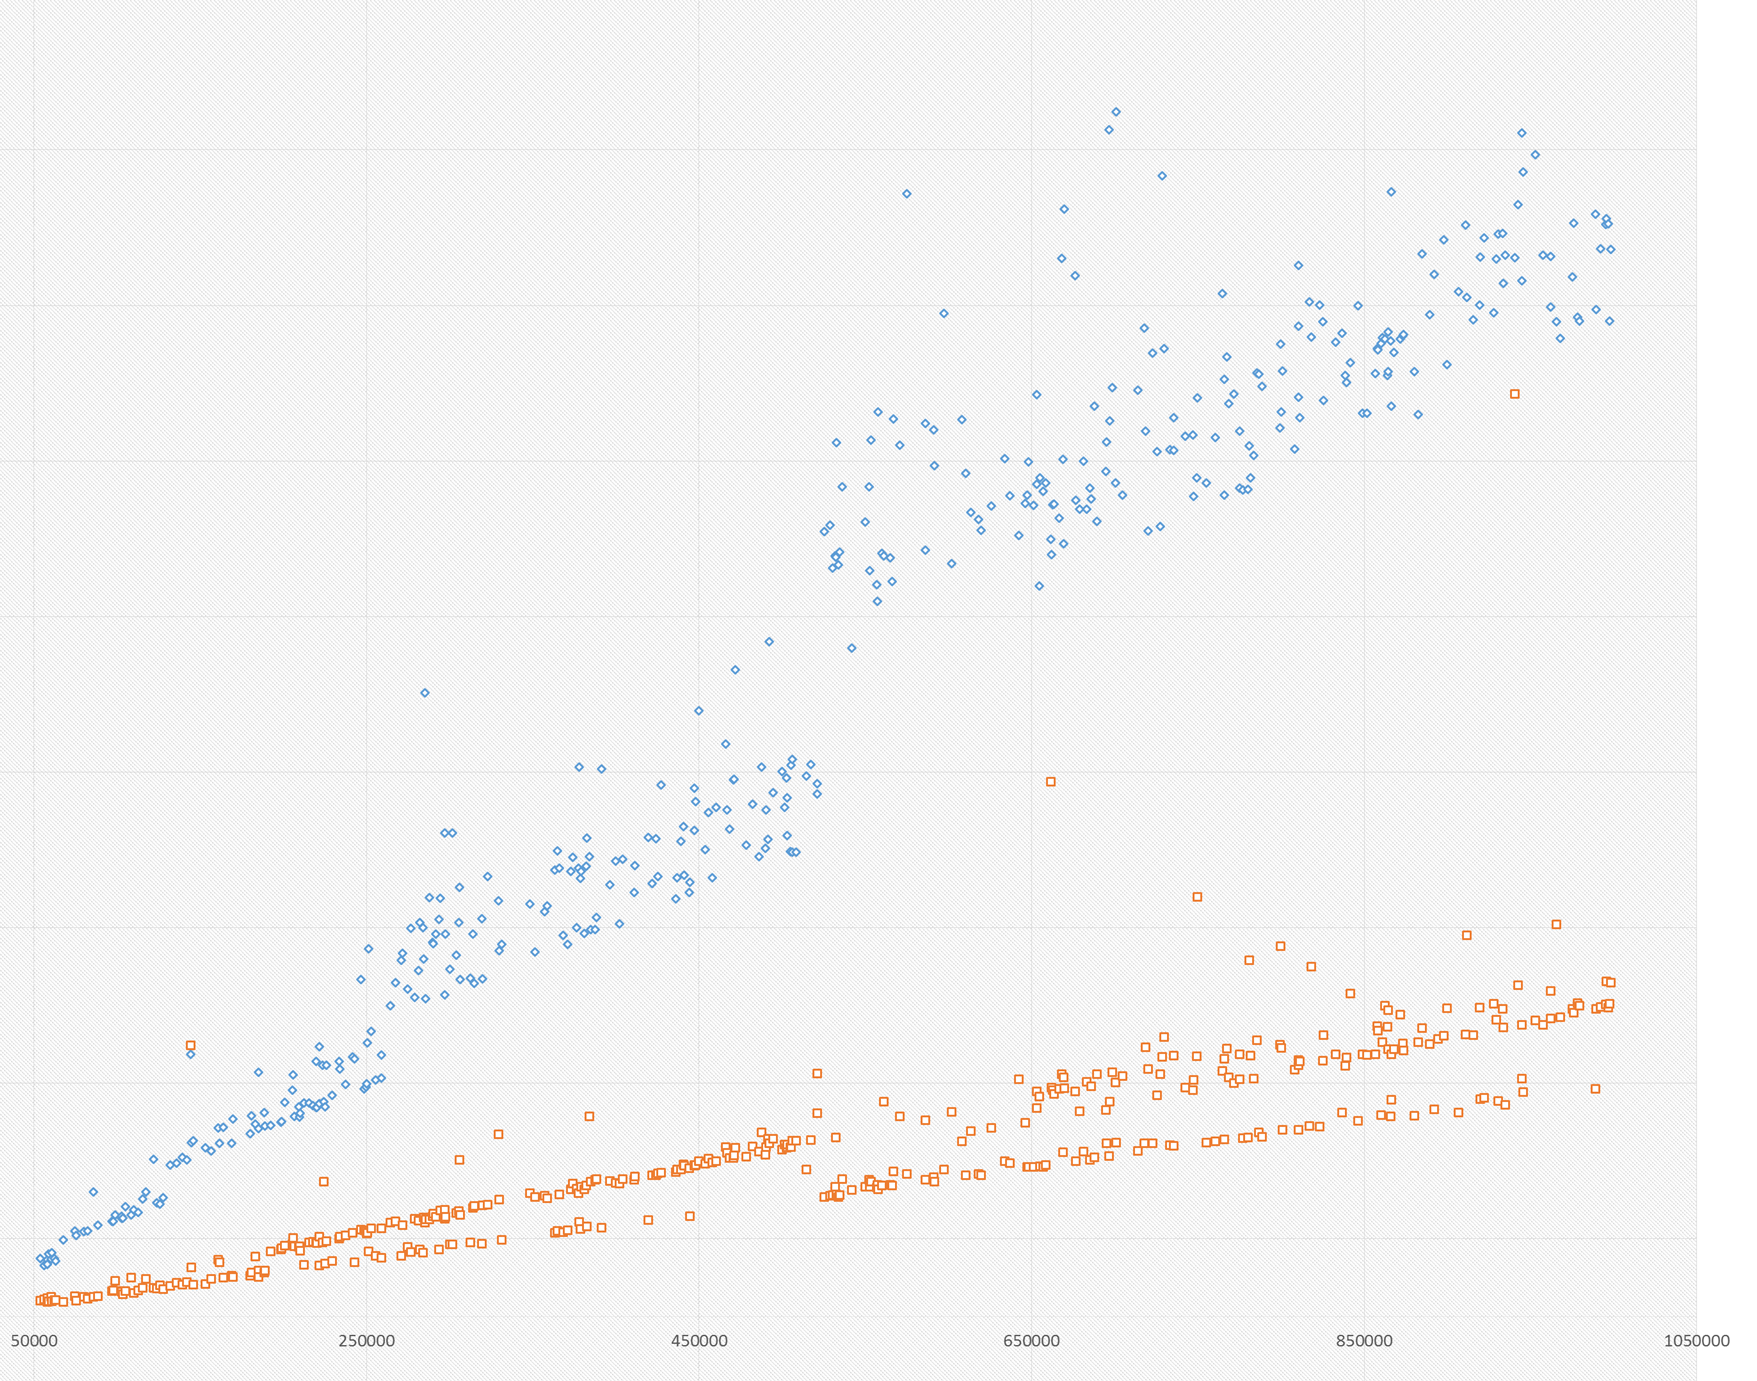
\includegraphics[width=1.1\textwidth]{dispersion.png}
\caption{Diagrama de dispersión de valores aleatorios , tiempo de inserción.}
\label{fig:dispersion}
\end{figure}
Aunque un diagrama de dispersión permite formarse una primera impresión muy rápida sobre el tipo de relación existente entre las dos variables, utilizarlo como una forma de cuantificar esa relación tiene un serio problema para nosotros pues en una situación ideal si tomáramos los puntos de la dispersión y los uniéramos debería darnos una linea recta, no tendríamos que preocuparnos de encontrar la recta que mejor se ajuste, pero en una nube de puntos dispersa como la presentada en la figura \ref{fig:dispersion}debemos realizar un ajuste. Realizar una regresión lineal para tener una mejor representación y modelo mas ajustado para el modelo es lo adecuado, además así se realiza en los laboratorios de física donde se busca un modelo mas acertado. 

Nuestra hoja de calculo posee estas herramientas ya incluidas por lo que haremos uso de ellas, que nos entrega la ecuación de la mejor linea recta como se puede ver en la figura \ref{fig:dispersion2}.
\begin{figure}[H]
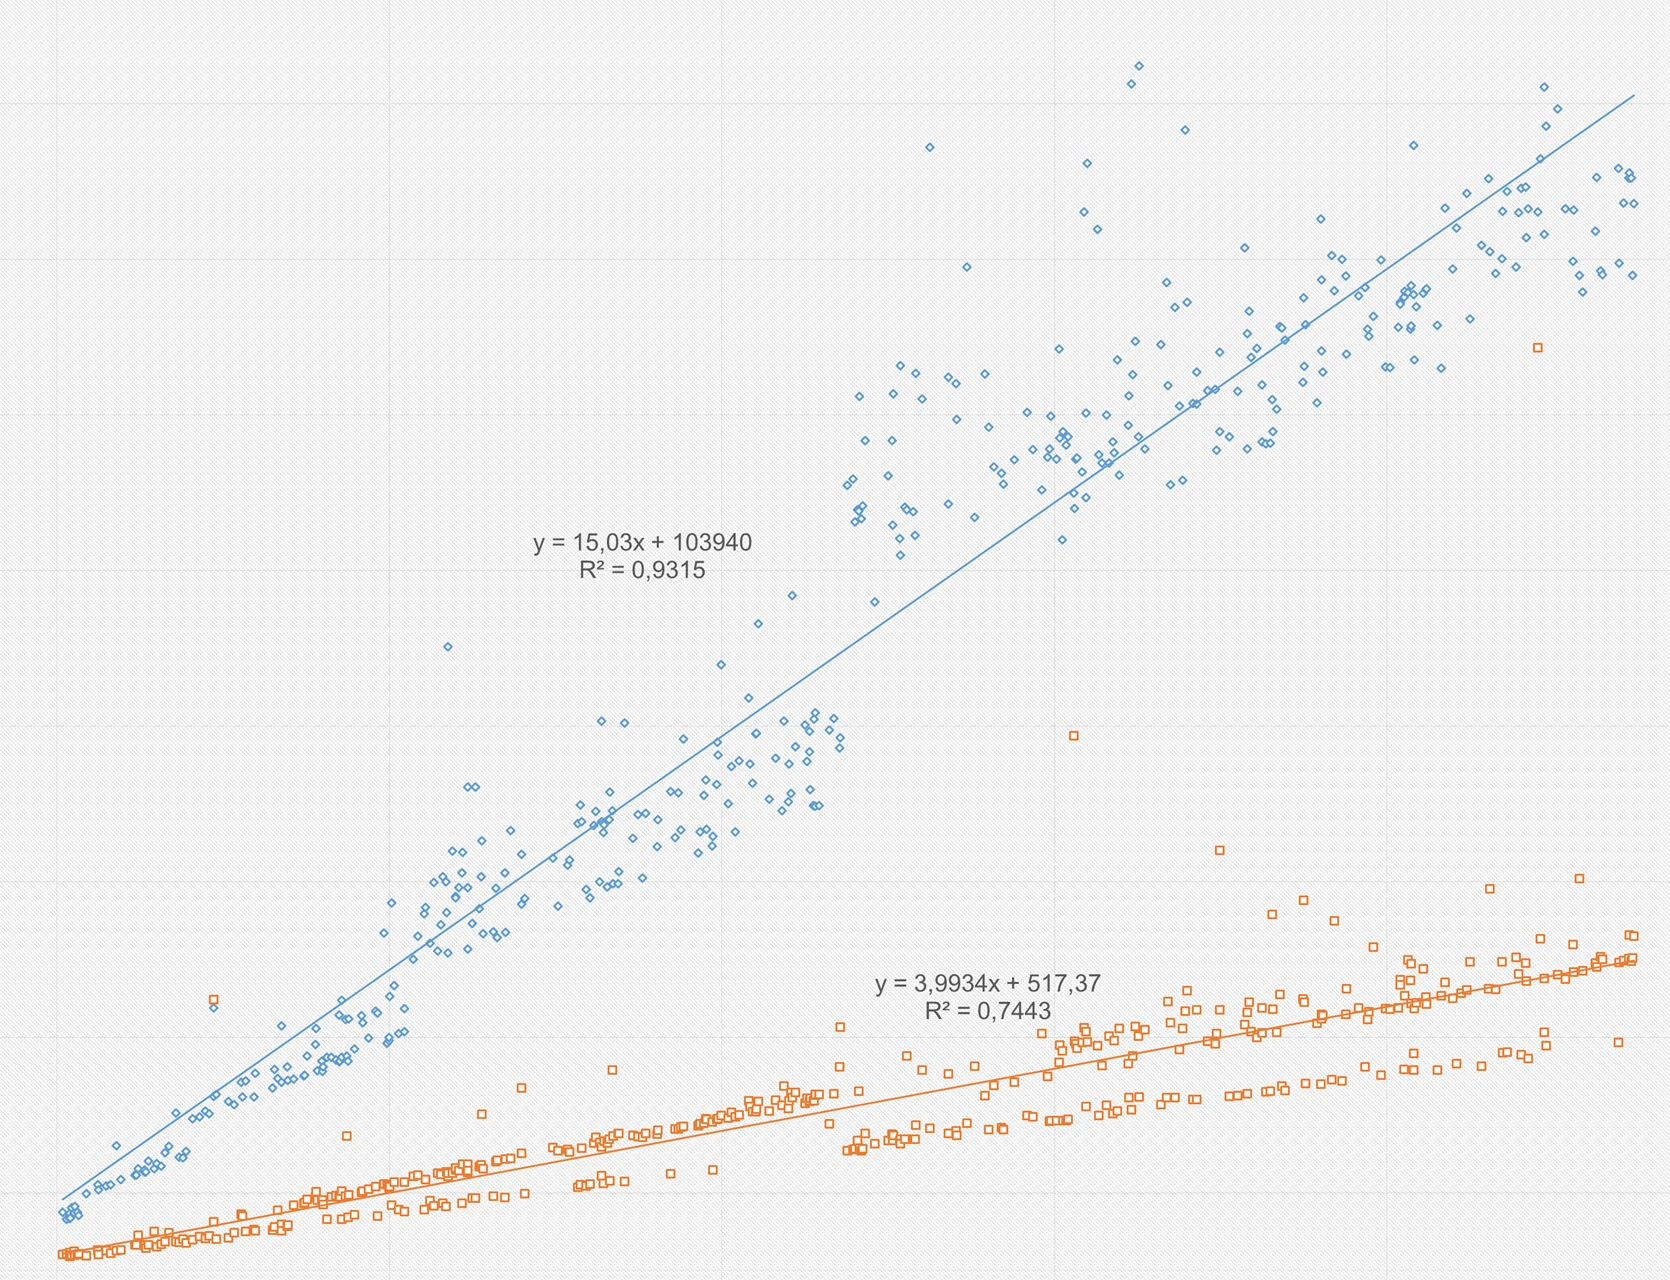
\includegraphics[width=1.1\textwidth]{dispersion2.png}
\caption{Regresión lineal.}
\label{fig:dispersion2}
\end{figure}
El $R^2$ indica cuanto porcentaje la Ecuación de la linea recta se aproxima en la relación de las variables, esto es un parámetro importante que nosotros hemos utilizado para aceptar o rechazar la ecuación que describe la relación de los datos.Nosotros hemos aceptado la representación 
\begin{figure}[H]
\includegraphics[width=1.1\textwidth]{multiples.png}
\caption{Gráfica de la Implementacion de Inserción para Vector y Array.}
\label{fig:multiples}
\end{figure}
Para comprobar que tan rápidos son los arrays y los vectores nosotros graficamos los datos que se ven en la figura \ref{fig:multiples} que presenta la comparación de 3 experimentos con un vector de 400 posiciones relleno de elementos aleatorios que describen el comportamiento de una distribución normal (o de Gauss) entre los rangos  $l=50000$ y $u=1000000$ , de los tres experimentos tenemos las siguientes valores promedio, y las siguientes desviaciones estandar:
\begin{table}[H]
\centering
\begin{tabular}{|c|l|l|}
\hline
\multicolumn{1}{|l|}{} & \multicolumn{1}{c|}{\textit{\textbf{\begin{tabular}[c]{@{}c@{}}Promedio de Valores\\ Aleatorios\end{tabular}}}} & \multicolumn{1}{c|}{\textit{\textbf{\begin{tabular}[c]{@{}c@{}}Desviacion Estandar \\ Valores Aleatorios\end{tabular}}}} \\ \hline
\textbf{Experimento 1} & 516974,105                                                                                                      & 271697, 05                                                                                                               \\ \hline
\textbf{Experimento 2} & 513338,9425                                                                                                     & 287655,06                                                                                                                \\ \hline
\textbf{Experimento 3} & 523706,3025                                                                                                     & 275309,08                                                                                                                \\ \hline
\end{tabular}
\caption{Promedios, y desviaciones estándar de los valores aleatorios del experimento de la figura 3.}
\label{desves}
\end{table}
Donde se puede observar que el valor promedio para el experimento1,experimento2,experimento3  de valores aleatorios es 518006 de 400 datos, con una desviación promedio de +-278220.4. El comportamiento linea salta a la vista de las gráficas pues era una de las cosas esperadas en el comportamiento. 

De la figura \ref{fig:multiples} se puede concluir que para los tres diferentes experimentos que se encuentran graficados en el mismo plano cartesiano, el comportamiento de sus homólogos tiene una tendencia muy parecida, en cuanto a la operación de inserción, los arrays son mucho mas eficientes respecto al tiempo, pues se puede observar que cuando el valor aleatorio a insertar es mayor en los arrays su tiempo es mucho menor comparado con la de los vectores.

Los arrays son estructuras de datos que no pueden expandir su tamaño de almacenamiento de forma dinámica por lo que tiene un tamaño fijo y nosotros como programadores debemos asegurarnos en resevar la memoria correspondiente a la cantidad de elementos que utilizaremos. insertar elementos en un array tiene una complejidad ($\mathcal{O}(n)$) con respecto al tamaño del array que estamos llenando, asumiendo que el array para llenarlo inicia en la posición \textbf{0}, es decir la operación de add para este punto siempre se va a realizar al final de la secuencia. Los vectores puede crecer dinamicamente, pero se debe realizar una operación de \textbf{resize} para nuestra prueba y solución de la pregunta 1.1 utilizamos la política por default de \textbf{ns=capacity*2}. Los datos según las figuras \ref{fig:multiples},\
\begin{figure}[H]
\includegraphics[width=0.9\textwidth]{p_ana1.png}
\caption{Experimento 2, n=1000}
\label{fig:ana1}
\end{figure}

\begin{figure}[H]
\includegraphics[width=0.9\textwidth]{p_ana11.png}
\caption{Diferencias, Experimento 1, n=1000}
\label{fig:ana2}
\end{figure}
Para nuestro segundo experimento decidimos incrementar el tamaño del vector que contendría los valores aleatorios por un \textbf{n=1000} \emph{véase figura \ref{fig:ana1},\ref{fig:ana2}}, Al tener mas datos nosotros como analistas y teniendo presente la \fnurl{teoría de los grandes números}{https://en.wikipedia.org/wiki/Law_of_large_numbers} podremos confiar mas en el comportamiento de los datos, como esto se trata de lidiar con datos y  probabilidades, esta ley establece que al observar continuadamente en el tiempo un experimento cuyo resultado es aleatorio los resultados tienden a estabilizarse. 
Podemos afirmar de nuestras practicas experimentales la implementacion de insercion mas rapida en tiempo es la de array para esta parte la addicion de un elemento 1 es al final de la secuecia. 
\subsubsection{VectorInsertion con Diferentes Políticas de Crecimiento}
Como sabemos la nuestra clase vector tiene una gran diferencia con respecto a 
\begin{itemize}
\item  int ns = capacity * 1.5;
\item  int ns = capacity * 1.8;
\item  int ns = capacity * 3;
\item int ns = capacity * 2;
\item int ns = capacity + 1;

\end{itemize} 

\begin{listing}[H]
	\begin{minted}{cpp}
 int ns = capacity + 1;
 int ns = capacity * 2;
 int ns = capacity * 3;
 int ns = capacity * 1.8;
 int ns = capacity * 1.5;
\end{minted}
\caption{Números Pseudo-aleatorios usando Merssene Twister}.
    \label{2nd:the-code}
\end{listing}





\section{Resultados}

\section{Conclusiones}

\section{Extras}
\section{Anexos}
El codigo para esta tarea se encuentra disponible en \texttt{github.com\/heticor915\/DataStructures\/Homeworks\/}
\end{document}
